% =====================================================================
%  [문서 구분]  이 파일 = IEEE IV 제출본 (국문 작업본)
%
%    docs/iv/iv_main_ko.tex  ← 이 파일. 국문으로 작성·유지한다.
%    docs/main.tex           ← 별개 문서. 박사학위논문(국문).
%
%  영문본(iv_main.tex)은 제거됨 — 영문 번역은 사용자가 직접 수행.
%  구 영문 초안: backup/docs/iv_main_en_20260915.tex
%
%  제출 조건(2026-09-16 공식 CFP 확인, ieee-iv.org/2027):
%    마감 2026-11-15, 기본 6쪽(그림·참고문헌 포함, 최대 8쪽+유료 2쪽),
%    저자 biography 불필요. 익명화는 제출 직전 사용자가 직접 처리(현재 실명).
%
%  컴파일: xelatex iv_main_ko.tex (한글 — pdflatex 아님). 이 환경엔 LaTeX 없음.
%
%  분량: 2026-09-16 2차 축약 후 Overleaf 실측 6쪽 확정(공식 기본 분량과 일치).
%    2차에서 줄인 것(수치는 전부 보존):
%      - 초록·서론·관련연구·방법·실험·고찰·결론 산문 압축
%      - stage 전이 표(구 tab:stage) 삭제 → 세 수치쌍을 학습 커리큘럼 본문에 인라인
%      - 고찰의 실패 개입 2개 단락을 1개 단락으로 병합(클래스 분석 중복 단락 제거)
%      - 참고문헌 45→34개(주변부 계보 인용 정리; references.bib 자체는 불변)
%      - 그림 1 폭 0.88\textwidth, 캡션 축약
%    ※ 수정(2026-09-28): 소거 표의 'w/o fusion'(게이트=0) 열 삭제 — 언어 없는 모델
%      행은 HiP-AD 논문 보고값으로 대체한다는 방침(사용자 지시 2026-09-21)에 따라
%      표 구성은 (a) 보고값 / (b) 어긋난 토큰 / (c) 융합 으로 통일.
%
%  ※ 해상도·체크포인트 표기: 본문의 모든 실측은 대표모델 s2hr(896x448, 2단계 완주)
%    한 체크포인트에서 나온다(표 1~5, 그림 1 제외 전부). 해상도를 '기여'로 쓰지 않는다.
%
%  ※ 2026-09-29 6쪽 축약: 그림2(게이트 분포)·그림3(클래스별 이득)·표(과제별 기여) 삭제
%    — 세 곳의 수치는 모두 본문 인라인으로 보존. 남은 플로트: 표1·2(2단), 표3·4·5(1단),
%    그림1(2단).
%
%  ※ 숫자 규칙: \measured{} = 실측값, \pending{} = 미확정값.
%    제출 전 \pending 이 하나도 남지 않아야 한다.
% =====================================================================
\documentclass[conference]{IEEEtran}
\IEEEoverridecommandlockouts

\usepackage{kotex}
\usepackage{cite}
\usepackage{amsmath,amssymb,amsfonts}
\usepackage{graphicx}
\usepackage{textcomp}
\usepackage{xcolor}
\usepackage{booktabs}
\usepackage{multirow}
\usepackage{url}

\newcommand{\measured}[1]{#1}
\newcommand{\pending}[1]{\textcolor{red}{\textbf{[미정:#1]}}}

\begin{document}

\title{LaQ-AD: Language-to-Query Fusion\\
for Sparse End-to-End Autonomous Driving}

\author{
\IEEEauthorblockN{Junhan Kim}
\IEEEauthorblockA{\textit{Graduate School of Automobile and Mobility} \\
\textit{Kookmin University} \\
Seoul, Republic of Korea \\
kimjunhan1605@gmail.com}
\and
\IEEEauthorblockN{Yeonsik Kang}
\IEEEauthorblockA{\textit{Department of Automotive Engineering} \\
\textit{Kookmin University} \\
Seoul, Republic of Korea \\
yeonsikkang@kookmin.ac.kr}
}

\maketitle

% =====================================================================
\begin{abstract}
Sparse query-based end-to-end driving models refine detection, online mapping,
motion forecasting and planning as one query pool in a shared decoder. Their
queries are grounded purely in geometry---each aggregates image features at
projected 3D locations---so context that is visible but not geometrically
salient, such as an occluded pedestrian implied by a stopped bus, has no path
into the representation. LaQ-AD injects the hidden token sequence of a
pretrained vision--language model (VLM) into that shared query pool through
cross-attention with a \emph{zero-initialized channel-wise gate}: the fused
model is identical to its unfused counterpart at step zero by construction,
and caching the VLM tokens offline keeps the VLM off the training critical
path. The same construction isolates
the language contribution without retraining---feeding each sample
\emph{another} sample's tokens costs \measured{1.7} detection mAP and
\measured{10.6} map mAP points, so the model acts on scene-specific language
content rather than on a learned constant. Gains concentrate on categories
whose identity is contextual: construction vehicle \measured{$+37$}\% and the
pedestrian-crossing map class \measured{$+41$}\% versus car \measured{$+1.4$}\%
(relative to the mismatched-token control; the rare-class bases are low, so
\measured{$+37$}\% is \measured{$+0.017$} AP). On nuScenes,
LaQ-AD reaches \measured{0.3967} detection mAP, \measured{0.4952} NDS,
\measured{0.5337} map mAP and \measured{0.3425} AMOTA. Code is available at
\url{https://github.com/KimJunHan/LaQ-AD}.
\end{abstract}

\begin{IEEEkeywords}
autonomous driving, end-to-end learning, vision--language models, 3D object
detection, multi-task learning
\end{IEEEkeywords}

% =====================================================================
\section{서론}
\label{sec:intro}

종단간 자율주행은 인지·예측·계획을 함께 학습하는 방향으로 수렴해
왔고~\cite{hu2023uniad,jiang2023vad}, 그중 \emph{희소 쿼리} 형식이 특히
효과적이다~\cite{sun2024sparsedrive,hipad2025}. 조밀한 조감도 격자 대신 고정된 수의
쿼리---주변 객체, 지도 요소, 자차---를 공유 디코더에서 정제하며, 각 쿼리는 자신의 3차원
앵커가 투영된 위치에서 영상 특징을 추출한다~\cite{lin2023sparse4dv3,zhu2021deformabledetr}.
이 효율은 하나의 가정 위에 서 있다. 각 쿼리는 자신의 앵커가 가리키는 위치의
영상만 본다는 것이다. 위치를 이미 아는 객체를 정밀하게 다듬는 데는 유리하지만, 그
위치에 \emph{보이지 않는} 맥락---정차한 버스 뒤에서 나타나려는 보행자, 20미터 앞 공사
표지 때문에 유효성이 달라지는 차선---을 알아채는 데는 오히려 불리한 구조다.

방대한 웹 데이터로 학습된 시각--언어 모델(VLM)은 3차원 정보 없이도, 영상 속 객체가
무엇이고 서로 어떤 관계이며 어떤 행동이 가능한지를 담은 토큰 열을
만든다~\cite{radford2021clip,wang2024qwen2vl}.
최근 주행 연구는 이를 주로 \emph{생성자}---VLM 이 궤적·서술·사고 연쇄를 내놓고 제어기가
소비하는 구조---로 사용해 왔는데~\cite{tian2024drivevlm,xu2024drivegpt4,sima2024drivelm},
이 구조는 VLM 의 느린 추론과 환각을 그대로 물려받고, 언어 모델을 오류를 점검하기 가장
어려운 파이프라인의 마지막 단에 두게 된다.

본 논문은 반대 방향을 택한다. VLM 에게 출력을 만들게 하는 대신, 주행 모델 내부의
특징에 언어 정보를 \emph{더해 주는} 역할만 맡긴다. VLM 의 은닉 토큰을 키·값으로, 주행
모델의 과제 쿼리를 질의로 하는 교차 어텐션을 두고, 그 출력에 게이트---언어
정보를 얼마나 반영할지 채널별로 정하는 학습 가능한 계수---를 곱해 잔차로 더하되, 이
게이트를 0 에서 출발시킨다(영초기화). 학습 시작 시점에는 게이트가 0 이라
언어가 전혀 더해지지 않으므로 모델은 기반 모델과 완전히 같고, 학습이 진행되면 언어가
도움이 되는 채널만 스스로 열린다. 학습 후 게이트를 도로 0 으로 잠그면 \emph{학습된
가중치의} 비융합 순전파가 즉시 복원된다---언어 없이 학습했을 모델과 같지는 않으므로,
본 논문은 이를 귀속의 상한이 아니라 통제의 출발점으로만 쓴다.

본 논문의 기여는 다음과 같다.
\begin{itemize}
  \item HiP-AD 위에 언어를 더한다. 기반 모델 HiP-AD~\cite{hipad2025}는 계획
        쿼리를 공간·시간·주행 스타일의 세 종류 waypoint 로 나눠(다중 granularity) 인지
        쿼리와 한 디코더 안에서 상호작용시켜 성능을 얻는 구조다. 본 논문은 이 구조를
        바꾸지 않고, 동결된 VLM 의 토큰을 교차 어텐션과 영초기화 게이트로 공유 쿼리 풀에
        주입하는 계층 하나만 추가한다. 토큰은 표본마다 미리 계산해 캐시하므로 학습 중
        VLM 을 실행할 필요가 없고 추가 비용은 $+0.66$M 파라미터에 그친다---단일 GPU
        학습과 차량 탑재의 연산 제약을 겨냥한 선택이다. 또한 언어는 행동·궤적을 직접
        생성하지 않는다---공유 쿼리 풀의 특징을 변조할 뿐이고 그 영향은 게이트로 끌 수
        있다. 다만 주입은 과제 분리 이전이라 계획·자차 쿼리에도 닿으므로, 언어가 인지
        경로만 거친다고 주장하지는 않는다.
  \item 언어의 효과를 재학습 없이 잰다. 융합은 구성상 초기화 시점에 항등($F'{=}F$)이고
        게이트를 $0$ 으로 두면 학습된 가중치의 비융합 순전파가 복원되므로, 한 번 학습한
        체크포인트 하나로 언어의 기여를 nuScenes 검출·매핑·추적에서 분리 측정할 수 있다.
        본 논문이 쓰는 통제는 어긋난 토큰이며, 잘못된 언어가 들어올 때의 거동(위치
        정밀도·재현율 동반 악화)까지 정량화한다.
  \item 롱테일 실패 지점을 찾아 진단한다. 크고 드문 두 범주(트레일러·공사차량)의
        낮은 성능이 클래스 혼동이 아니라 \emph{검출 실패}임을 보이고, 트레일러의 경우
        그 실패가 거리에 따라 나타나---앵커 크기가 전부 같아 먼 대형차를 작은 발자국으로
        훑는 구조적 문제와 일치함을---재현 가능한 절차로 제시하며, 언어 이득이 정확히 맥락 의존적
        희소 범주에 집중됨(공사차량 $+37$\%)과 실패한 네 개입을 그대로 보고한다.
\end{itemize}

단순 결합과의 차이. 본 설계는 HiP-AD 에 언어 모델을 이어 붙인 것과 세 지점에서
다르다. 첫째, \emph{역할}이 다르다. 기존 주행용 VLM
연구~\cite{tian2024drivevlm,xu2024drivegpt4,sima2024drivelm}는 VLM 이 궤적·서술을
생성해 제어에 직접 관여하지만, 본 설계의 VLM 은 텍스트를 한 글자도 생성하지 않는다.
은닉 토큰이 표현 수준에서만 주입되므로 잘못된 언어의 영향이 게이트로 감쇠되고, 그
영향의 크기까지 실험으로 정량화된다(\ref{sec:ablation}절). 둘째,
\emph{주입 지점}이 다르다. 계획기 하나가 아니라 단일 디코더의 공유 쿼리 풀에 각 계층
내부에서 주입되어 검출·지도·계획이 같은 언어 신호를 공유한다---본 설정에서 매핑의
상대 이득이 검출의 \measured{5.7}배다. 셋째, \emph{결합 자체가 측정 장치}다.
영초기화 게이트와 결정적 오프라인 캐시 덕분에 ``언어만 뺀 같은 모델''을 재학습 없이
복원할 수 있다---VLM 이 생성한 출력이 제어에 섞여 들어가는 결합에서는 성립하지 않는
성질이다.

% =====================================================================
\section{관련 연구}

카메라 전용 3차원 인지는 조밀 조감도 격자~\cite{philion2020lss,li2022bevformer}에서
쿼리 기반 형식~\cite{wang2022detr3d,wang2023streampetr}으로 이동해 왔고,
Sparse4D~\cite{lin2023sparse4d,lin2023sparse4dv3}가 앵커별 키포인트에 대한 가변형
집약과 인스턴스 단위 시간 전파로 이를 발전시켰다---본 논문 디코더의 추출 기제이자
\ref{sec:anchors}절에서 크기 제약을 보이는 대상이다. 다중 과제 방향에서는
UniAD~\cite{hu2023uniad}와 VAD~\cite{jiang2023vad}가 인지·예측·계획의 공동 학습을
확립했고, SparseDrive~\cite{sun2024sparsedrive}가 조밀 부호화기를 제거했으며,
HiP-AD~\cite{hipad2025}가 공유 쿼리 풀 위의 단일 디코더로 통합했다---본 논문의 기반
구조다. 후속 연구~\cite{weng2024paradrive,jia2025drivetransformer,liao2025diffusiondrive}와
벡터화 매핑~\cite{liao2023maptr}도 같은 계보이며, 이 계보의 쿼리는 모두 DETR 의 집합 예측~\cite{carion2020detr}을 따르며, 오직
기하(앵커 위치)에만 근거해 영상을 참조한다. 한편 주행용 VLM
연구~\cite{xu2024drivegpt4,tian2024drivevlm,sima2024drivelm}는 VLM 을 추론 엔진으로,
주행 스택을 그 실행자로 다룬다. 본 논문의 사용은 더 좁다. VLM 은 제어기에 도달하는
행동·궤적을 결코 생성하지 않고, 기하에 묶인 디코더가 학습된 게이트로 줄이거나 무시할 수 있는
맥락 특징만 공급한다. 영초기화 게이트 자체는 사전학습 신경망을 훼손 없이 확장하는 확립된
방식~\cite{llamaadapter2023}이다. 본 논문의 기여는 이 구성이 안정화 장치일 뿐 아니라,
다중 과제 주행에서 \emph{언어의 효과를 따로 측정하는 실험 도구}가 된다는 관찰이다.

% =====================================================================
\section{방법}
\label{sec:method}
그림~\ref{fig:arch}이 전체 구조를 보인다.

\begin{figure*}[t]
\centering
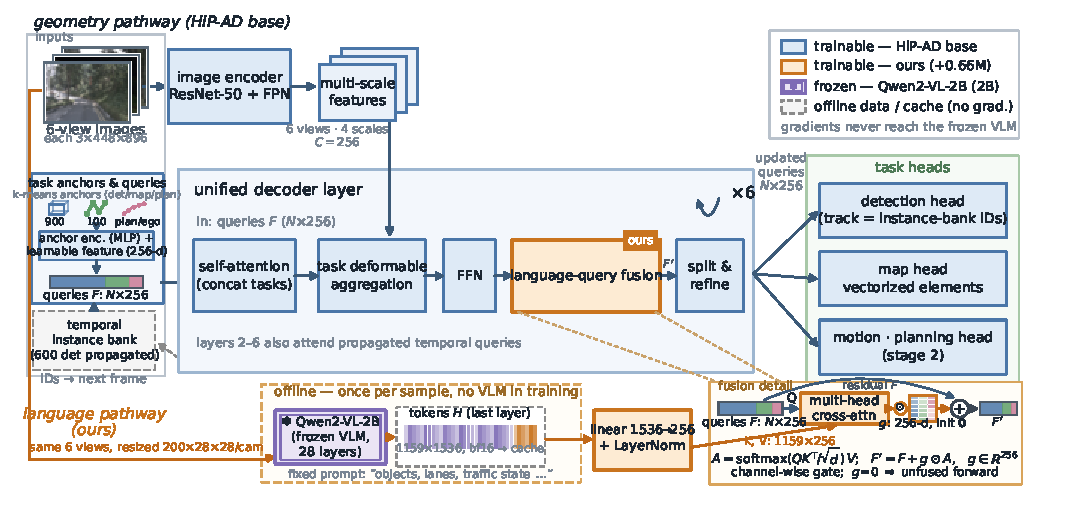
\includegraphics[width=\textwidth]{figures/architecture.pdf}
\caption{LaQ-AD 개요. 기하 경로(상단·중앙)는 기반 구조~\cite{hipad2025} 그대로다---
공유 쿼리 풀(객체 900·지도 100·계획/자차)이 통합 디코더 계층($\times6$)에서 6방향 영상
특징을 가변형 집약으로 참조하고, 시간적 인스턴스 뱅크가 검출 쿼리 600개를 다음 프레임으로
전파한다(트랙 ID 의 근거). 본 논문의 추가분은 \emph{각 디코더 계층 내부}, 집약·FFN
뒤·과제 분리 전에 삽입된 언어 교차 어텐션이다(하단). 같은 6방향 영상과 고정
지시문을 동결된 Qwen2-VL-2B~\cite{wang2024qwen2vl}에 넣어 얻은 중간 계층(18층) 은닉
토큰열을 표본마다 한 번 오프라인 캐시하고, 2층 MLP 사영을 거쳐 K·V 로 공급하며,
계층$\times$과제$\times$채널로 분해된 영초기화 게이트 잔차로 더한다---학습 0단계의
출력은 기반 모델과 동일하며, VLM 은 학습 중 한 번도 실행되지 않는다.}
\label{fig:arch}
\end{figure*}

\subsection{준비: 공유 쿼리 풀}
단일 디코더 희소 구조~\cite{hipad2025}를 기반으로 한다. 주변 객체 쿼리 $900$개, 지도
쿼리 $100$개, 자차·계획 쿼리로 구성되며 각 쿼리는 인스턴스 특징
$f_i\in\mathbb{R}^{256}$ 과 앵커(객체는 3차원 상자, 지도는 폴리라인)를 지닌다. 디코더 한
계층은 과제별 쿼리를 이어 붙여 자기 어텐션을 적용하고, 앵커에서 생성된 키포인트 위치의
다중 시점 영상 특징을 가변형 집약으로 추출하며, 전방향 신경망을 거쳐 풀을 나누고 앵커를
정제한다. 여섯 계층이 쌓이고 뒤쪽 계층은 시간적 인스턴스 뱅크로 전파된 쿼리(검출 900개
중 600개)에도 어텐션한다. 시간 전파가 유효하도록 학습 배치는 장면 단위 그룹 샘플러로
연속 프레임을 묶고 같은 시퀀스에 동일한 증강을 적용한다. 분류는 focal
손실~\cite{lin2017focal}, 상자 회귀는 L1, 매칭은 헝가리안
알고리즘~\cite{kuhn1955hungarian}을 따른다.

\subsection{오프라인 시각--언어 토큰 캐시}
시각 $t$ 의 6방향 영상을 사전학습된 Qwen2-VL-2B~\cite{wang2024qwen2vl}에 고정
지시문---``전방·전좌·전우·후좌·후·후우 6방향 서라운드 영상이다. 두드러진 객체, 차선
기하, 교통 상태, 주행에 유관한 단서를 서술하라''---과 함께 입력해 표본마다 한 번
실행하고, 은닉 상태 $H_t \in \mathbb{R}^{L \times d_{\text{vlm}}}$ ($L{=}1159$,
$d_{\text{vlm}}{=}1536$)을 \texttt{bfloat16} 으로 저장한다. 영상은 카메라당
$200{\times}28{\times}28$ 화소 예산으로 고정 리사이즈되어(시각 토큰은 병합 후 카메라당
$180$개) 토큰 길이가 일정하고, 지시문이
고정이므로 캐시는 결정적이다. 본 논문이 보고하는 모델은 마지막 계층의 은닉 상태를 쓴다. 순전파 한 번에 전 계층이
계산되므로 중간 계층(14·18·22층)도 같은 비용에 저장해 두었으나, 어느 계층이 융합에
유리한지는 본 논문의 평가 범위 밖이며 후속 작업으로 남긴다. VLM 과 입력이 고정이므로 $H_t$ 는 에폭에
따라 변하지 않는다. 전체 데이터셋에 한 번 계산해 두고(nuScenes 기준 $34{,}149$개 텐서,
$114$\,GB) 학습 중에는 디스크에서 읽으므로 학습 루프는 VLM 을 인스턴스화하지 않는다.
캐싱은 VLM 을 주행 과제에 맞춰 미세조정할 가능성을 스스로 막는 의도적 제약이다. 그
대가로 100 에폭 일정을 단일 GPU 에서 소화할 수 있고, 모든 비교 설정에 정확히 같은
언어 신호가 들어감이 보장된다.

\subsection{영초기화 게이트를 둔 언어--쿼리 교차 어텐션}
디코더의 어느 계층에서 전체 쿼리 풀의 인스턴스 특징을
$F \in \mathbb{R}^{B \times N \times d}$, 해당 표본의 캐시된 VLM 토큰을 $H$ 라 하자.
$H$ 를 선형 사영($1536\!\to\!256$)과 LayerNorm 으로 정렬한 뒤 $A = \mathrm{MHA}(Q{=}FW_q,\, K{=}HW_k,\, V{=}HW_v)$ 를 메모리 효율적
어텐션~\cite{dao2022flashattention}으로 계산한다. 융합 출력은 \emph{게이트가 걸린
잔차}이며, 게이트는 채널별로 학습되는 0 초기화 벡터다(0 초기화 잔차 게이트는
LLaMA-Adapter 의 zero-init attention~\cite{llamaadapter2023}과 같은 계보다):
\begin{equation}
  F' = F + g \odot A, \qquad
  g \in \mathbb{R}^{d},\;\; g^{(0)} = \mathbf{0},
  \label{eq:gate}
\end{equation}
어느 채널에 언어를 얼마나 받아들일지는 학습이 결정하게 하고, 학습된 $g$ 의 분포를 분석
결과로 삼는다(\ref{sec:ablation}절). 같은 형식은 디코더 계층과 과제 축으로도 일반화되지만
($g \in \mathbb{R}^{L\times S\times d}$), 본 논문이 보고하는 수치는 모두 채널 축 형태에서
나온 것이며 분해 게이트의 평가는 후속 작업이다. 식~\eqref{eq:gate}은 두 결과를 낳는다.
초기화 시점에 $F' = F$ 가 정확히 성립해 융합·비융합 모델이 같은 함수이고, 이후 어느
시점이든 $g{=}0$ 으로 두면 \emph{학습된 가중치의} 비융합 순전파가 복원된다---게이트는
안정화 장치이자 측정 도구다(\ref{sec:ablation}절). 계층은 가변형 집약과 전방향 신경망
뒤, 풀이 과제별로 나뉘기 \emph{전}에 삽입한다---언어가 영상에서 이미 추출된 특징을 변조하고, 한
계층이 네 과제 쿼리에 동시에 닿는다.

\subsection{학습 커리큘럼}
선행 연구~\cite{sun2024sparsedrive,hipad2025}를 따라 인지를 먼저, 모션을 뒤에 학습한다.
1단계(인지)는 검출과 온라인 매핑을 지도학습하며, 계획·자차 쿼리는 디코더 구성을
최종 모델과 일치시키기 위해 풀에 존재하되 손실 가중치를 0 으로 둔다. 100 에폭, 유효 배치
$64$, AdamW~\cite{loshchilov2019adamw} $2\!\times\!10^{-4}$, 코사인
감쇠~\cite{loshchilov2017sgdr}와 $500$ 스텝 준비 구간을 쓴다. 보고하는 모델의 1단계는
$704\!\times\!256$ 에서 이 일정을 마친 뒤 $896\!\times\!448$ 로 $12$ 에폭 미세조정한
것이다(같은 해상도로 처음부터 학습하는 일정은 진행 중이다). 2단계(모션)는
모션 쿼리·손실과 계획·자차 손실을 켜고 1단계 가중치에서 시작한다(10 에폭, 유효 배치
$48$, 입력 해상도는 1단계와 동일). 이 전환을 아무 보정 없이---모든 파라미터를 1단계의 최고 학습률로 되돌리고 모션 손실을
기본 가중치 그대로 두고---수행하면 인지 성능이 크게 떨어짐을 관측했다: 검출 mAP \measured{$-4.9$}\%, 지도 mAP
\measured{$-3.0$}\%, AMOTA \measured{$-23.7$}\%. 원인을 분해해 두 가지를 수정하면
같은 데이터·평가에서 \measured{$+1.0$}\%/\measured{$-0.2$}\%/\measured{$-1.5$}\% 로
회복된다. (i) 기준 학습률을 $2\!\times\!10^{-5}$ 로 낮추고 신규 모션 모듈에만 배수를 주어
유효 $2\!\times\!10^{-4}$ 로 맞춘다---100 에폭에 걸쳐 도달한 수렴점을 큰 학습률이 흔드는
것을 막는다. (ii) 모션 회귀 손실 가중치를 절반으로 낮춘다. 기본값은 지평 $6$ 스텝 기준인데
nuScenes 는 $12$ 스텝이고 손실이 지평으로 나눠지지 않아, 그대로 두면 공유 특징이 모션
쪽으로 쏠린다.

모든 학습은 \texttt{fp32} 로 수행한다. 혼합 정밀도~\cite{micikevicius2018mixed}에서는 어텐션
내부에서 fp16 범위를 넘는 값이 생겨 수만 반복 뒤 분류 출력이 NaN 이 되었다. 동적 손실
스케일링과 스텝 건너뛰기는 넘침을 가릴 뿐이라 채택하지 않았고,
해당 경로를 전 정밀도로 유지해 넘침 자체를 없앴다.

\subsection{평가 산출 프로토콜}
검출·매핑은 각 헤드의 출력을 그대로 평가하며, 검출은 분류 점수 상위 300개를 표본당
제출한다. \emph{추적은 별도 모듈 없이} 시간적 인스턴스 뱅크가 프레임 간에 유지하는
인스턴스 식별자를 트랙 식별자로 쓰는 후처리라 어느 단계의 체크포인트로도 산출된다. 트랙 제출의 점수 임계값 $0.15$ 는 검증 분할에서 선택했으며, 보고 모델의 AMOTA 는
$0.10$/$0.15$/$0.20$ 에서 각각 \measured{0.3255}/\measured{0.3425}/\measured{0.3274}
다---선택값이 최댓값이므로 이 수치는 검증 분할에 맞춰 조정된 운용점임을 밝혀 둔다(기준
문헌의 임계값은 공개되어 있지 않다).

\subsection{단일 체크포인트 소거 프로토콜}
\label{sec:onerun}
본 설계의 부산물로, 언어 경로에 대한 소거가 \emph{한 번의 학습에서 나온 체크포인트
하나}로 산출된다(표~\ref{tab:negative}의 구조 개입들은 별도 학습이 필요한 비교로, 여기
해당하지 않는다).
게이트가 0 초기화 잔차이므로 (i) 영점화 = 학습된 가중치의 비융합 순전파가 재학습 없이
복원되고, (ii) 어긋난 토큰 통제는 캐시 파일명을 뒤섞되 어떤 표본도 자기 토큰을 받지 않는
순열로 재연결해 모든 표본이 다른 장면의 토큰을 받게 구성한다. 각각 검증 분할 추론 1회의
비용이며 새 학습은 없다. 본 논문이 보고하는 통제는 (ii)다---(i)은 학습 중 언어에 맞춰진
가중치를 그대로 두고 경로만 끄는 것이라 언어 없이 \emph{학습된} 모델과 동등하지 않으므로,
무언어 기준으로는 공개된 기반 모델의 보고값(표~\ref{tab:ablation}(a))을 쓴다.
구현상 캐시 적재는 실패를 숨기지 않는다---캐시가 없는 표본을 조용히 건너뛰면 일부 표본만
언어 없이 학습되어 소거 비교 자체가 성립하지 않으므로 즉시 실패시킨다.

% =====================================================================
\section{실험}

\subsection{설정}
nuScenes~\cite{caesar2020nuscenes}(전체 \texttt{v1.0-trainval}, 학습 \measured{28{,}130}
표본, 검증 \measured{6{,}019} 표본)에서 평가한다. ResNet-50~\cite{he2016resnet} 백본과
FPN~\cite{lin2017fpn} 넥, $896\!\times\!448$ 입력, per-GPU 배치와 기울기 누적으로 유효 배치를
구성하며(1단계 $8\times8=64$, 2단계 $4\times12=48$), 그 외 학습 일정과 손실 구성은~\cite{hipad2025}의 nuScenes
프로토콜을 따른다. 모든 실험은 단일 GPU 에서 수행했다.

\subsection{주요 결과}

% 갱신(2026-09-28): 본문의 모든 실측(주요결과·소거·과제별·클래스별·두 그림)을
%   대표모델 s2hr(2단계 완주, 896x448) 한 체크포인트에서 재산출해 교체 완료.
%   AMOTA·추적 지표는 논문 프로토콜(임계 0.15), minADE 는 car/ped 평균(0.674/0.757).
\begin{table*}[t]
\caption{Open-loop results on the nuScenes validation split (\measured{6{,}019}
samples). Baseline rows are reproduced from the comparison in~\cite{hipad2025};
all are final models trained through both stages. Our backbone and schedule match the
baseline but the input size differs ($896\!\times\!448$); our claim rests on
the within-pipeline comparison of Table~\ref{tab:ablation}.}
\label{tab:main}
\centering
\small
\begin{tabular}{lccccc}
\toprule
\multirow{2}{*}{Method} & \multicolumn{2}{c}{Detection} & Map & Track & Motion \\
\cmidrule(lr){2-3}\cmidrule(lr){4-4}\cmidrule(lr){5-5}\cmidrule(lr){6-6}
 & Det.\ mAP$\uparrow$ & NDS$\uparrow$ & Map mAP$\uparrow$ & AMOTA$\uparrow$ & minADE$\downarrow$ \\
\midrule
UniAD~\cite{hu2023uniad}                & 0.380 & 0.359 & --    & --    & -- \\
VAD~\cite{jiang2023vad}                 & 0.276 & 0.397 & 0.476 & --    & -- \\
SparseDrive-S~\cite{sun2024sparsedrive} & 0.418 & 0.525 & 0.551 & 0.386 & 0.62 \\
DiFSD~\cite{su2024difsd}                & 0.410 & 0.528 & 0.560 & --    & -- \\
HiP-AD~\cite{hipad2025}                 & 0.424 & 0.535 & 0.571 & 0.406 & 0.61 \\
\midrule
LaQ-AD (ours)
  & \measured{\textbf{0.3967}} & \measured{\textbf{0.4952}} & \measured{0.5337}
  & \measured{\textbf{0.3425}} & \measured{0.716} \\
\bottomrule
\end{tabular}
\end{table*}

표~\ref{tab:main}이 비교 결과다. 본 모델은 공개된 기준에 못 미치며, 유리한 부분만 고르지
않고 이를 그대로 밝힌다. 이 격차를 해석할 때는 두 가지 사실을 함께 보아야 한다.
첫째,~\cite{hipad2025}의 nuScenes 데이터 경로는 공개된 적이 없다---공개된 것은
Bench2Drive 쪽뿐이다. 모델 자체는 정확히 재현했으나(검출 앵커 900·시간 전파 600·감쇠
$0.6$·분류--회귀 임계 $0.05$·단일 프레임 디코더 1·지도 앵커 100 등 구조 하이퍼파라미터
전부 일치 확인) 데이터셋 변환, 정답 구성, 앵커 생성, 지도 평가기는 우리가 직접 다시 구현한 것이다.
둘째, 이 격차는 언어 경로와 무관하다---언어는 우리가 측정한 모든 설정에서 성능을
\emph{더한다}(\ref{sec:ablation}절). 입력을 $2.23$배로 올리면 검출 mAP 가
\measured{4.3}\%, AMOTA 가 \measured{16.3}\% 회복되고 이득은 작거나 세로로 긴 범주에
집중되며(자전거 \measured{$+16.9$}\%, 버스 \measured{$+9.9$}\%), 매핑만 이득이
없다(\measured{$-0.6$}\%).

\subsection{소거 실험: 언어 경로의 기여}
\label{sec:ablation}

\begin{table*}[t]
\caption{\textbf{Core evidence.} (a) is the published number of the base
model. (b) and (c) use \emph{identical} trained weights and differ only at
inference: (b) keeps the fusion pathway active but feeds each sample another
sample's cached tokens, corrupting the language \emph{content} while
preserving its statistics. If the gate had merely learned a useful constant
bias, (b) would match (c). $\Delta$(c$-$b) and $\Delta$(c$-$a) measure
different things---a within-checkpoint effect and a reproduction gap---and
must not be added or cancelled (Sec.~\ref{sec:discussion}). Rows (b) and (c)
come from the same final two-stage checkpoint as Table~\ref{tab:main}; AMOTA
uses the protocol threshold ($0.15$).}
\label{tab:ablation}
\centering
\small
\begin{tabular}{llcccc}
\toprule
 & Setting & Det.\ mAP$\uparrow$ & NDS$\uparrow$ & Map mAP$\uparrow$ & AMOTA$\uparrow$ \\
\midrule
(a) & HiP-AD~\cite{hipad2025} (base model, reported)
  & 0.424 & 0.535 & 0.571 & 0.406 \\
(b) & mismatched tokens --- pathway on, content wrong
  & \measured{0.3801} & \measured{0.4830} & \measured{0.4276} & \measured{0.3344}\\
(c) & correct tokens --- LaQ-AD as deployed
  & \measured{\textbf{0.3967}} & \measured{\textbf{0.4952}}
  & \measured{\textbf{0.5337}} & \measured{\textbf{0.3425}}\\
\midrule
  & $\Delta$ (c$-$b)\quad scene-specific content
  & \measured{$+$0.0166} & \measured{$+$0.0122}
  & \measured{$+$0.1061} & \measured{$+$0.0081}\\
  & $\Delta$ (c$-$a)\quad vs.\ reported base
  & \measured{$-$0.0273} & \measured{$-$0.0398}
  & \measured{$-$0.0373} & \measured{$-$0.0635}\\
\bottomrule
\end{tabular}
\end{table*}




먼저, 학습은 게이트를 닫아 두지 않았다---0 에서 출발한 \measured{256}개 채널 \emph{전부}가 0 을 벗어났고(음수
\measured{134}·양수 \measured{122}), 분포는 0 주변이 비고 양쪽에 봉우리가 선 이봉
형태다. 채널마다 다른 방향·크기를 학습했고, 0 으로 남을 수 있었음에도 그러지 않았다.

표~\ref{tab:ablation}의 (b)는 융합 경로·게이트·가중치를 그대로 두고 \emph{어느} 표본의
토큰이 도착하는지만 바꾼다. 게이트가 장면과 무관한 상수를 더하도록 학습된 것뿐이라면 (b)는
(c)와 같아야 하지만, 네 지표 모두에서 (b)가 낮다---검출 mAP \measured{$-0.0166$}, 지도
mAP \measured{$-0.1061$}. 어긋난 토큰은 추적 매칭쌍의 위치 정밀도(MOTP
\measured{$0.6577$}$\to$\measured{$0.6819$})와
재현율(\measured{$0.4522$}$\to$\measured{$0.4395$})을 함께 악화시키고, 지도 요소별로도
횡단보도 \measured{0.4781}$\to$\measured{0.3392}, 차선 \measured{0.5636}$\to$\measured{0.4673},
경계 \measured{0.5595}$\to$\measured{0.4762} 로 일관되게 떨어진다.
더 엄격한 운용점(임계 $0.2$)에서는 프레임당 오경보가 \measured{$31.1$} 에서
\measured{$97.1$} 로 3배가 되어 틀린 서술이 함의하는 객체를 환각하는 거동이 드러나지만,
이 지표는 운용점에 민감해 근거로 삼지는 않는다. 즉 모델은 어긋난 언어를 무시하지 않고
그에 따라 행동한다---융합 특징이 장면마다 다른 내용을 담을 때만 가능한 거동이다. 클래스별·과제별
이득의 구조는 \ref{sec:discussion}절에서 논한다.

\subsection{남은 격차의 소재}

\begin{table}[t]
\caption{Per-class detection AP and true-positive errors. Two rare categories
sit an order of magnitude below the rest and account for most of the aggregate
gap.}
\label{tab:perclass}
\centering
\small
\begin{tabular}{lcc@{\hskip 8pt}lc}
\toprule
Class & AP$\uparrow$ & AOE$\downarrow$ & Metric & Value \\
\midrule
traffic cone & \measured{0.674} & --               & mATE & \measured{0.6117}\\
car          & \measured{0.638} & \measured{0.105} & mASE & \measured{0.2806}\\
barrier      & \measured{0.586} & \measured{0.214} & mAOE & \measured{0.5781}\\
pedestrian   & \measured{0.505} & \measured{0.682} & mAVE & \measured{0.3080}\\
motorcycle   & \measured{0.407} & \measured{0.897} & mAAE & \measured{0.2524}\\
bicycle      & \measured{0.401} & \measured{1.213} &      & \\
truck        & \measured{0.317} & \measured{0.183} &      & \\
bus          & \measured{0.305} & \measured{0.146} &      & \\
trailer      & \measured{0.070} & \measured{0.582} &      & \\
constr.\ veh.& \measured{0.064} & \measured{1.181} &      & \\
\bottomrule
\end{tabular}
\end{table}

표~\ref{tab:perclass}은 남은 격차가 산발적이지 않음을 보인다. 첫째, 트레일러
(\measured{0.070})와 공사차량(\measured{0.064})이 나머지 여덟 범주
(\measured{0.305}$\sim$\measured{0.674})보다 한 자릿수 낮다. 이 둘만 $0.21$ 이어도 검출 mAP
\measured{0.425}, 두 범주를 제외하면(TP 오차도 나머지 여덟 범주로 재계산) 검출 mAP
\measured{0.4792} / NDS \measured{0.5528}
다(격차가 두 범주에 몰려 있음을 보이기 위한 수치이지 타 모델과의 비교치가
아니다---기준 문헌은 클래스별 수치를 공개하지 않는다). \emph{희소성}은 설명이 안 된다---트레일러 \measured{20{,}701}개는
자전거 \measured{9{,}478}개보다 흔한데 점수는 \measured{5.7}배 낮다. \emph{주석 손실}도
아니고(상자 치수 중앙값이 데이터셋 통계와 일치) \emph{변환 필터링}도 아니다(유효성
플래그 제거율 트레일러 \measured{3.6}\% < 승용차 \measured{11.3}\%). 둘째, 맞힌 상자들 중에서는 방향(요각) 오차가 가장 크다---mAOE \measured{0.5781}, 자전거 \measured{1.213}, 공사차량
\measured{1.181}.
$\mathrm{NDS}=\frac{1}{10}\bigl(5\,\mathrm{mAP}+\sum_{\mathrm{TP}}(1-\min(1,e))\bigr)$
이므로 검출 mAP 를 $0.424$ 로, mAOE 를 $0.35$ 로 개선하면
$\mathrm{NDS}=\measured{0.532}$ 로 목표선에 근접하며, 남은 차이는 위치 오차(mATE
\measured{0.6117})에서 온다. 총 격차는 모델 전반에 퍼져 있지 않고 희소
클래스 재현율과 요각 추정에 집중되어 있다.

\begin{table}[t]
\caption{Fraction of ground-truth boxes with a same-class prediction within
$2\,$m, by ego distance (validation split, same checkpoint as
Table~\ref{tab:main}; $n$ in parentheses). Trailers are found as reliably as
cars up close and then fall away; construction vehicles are poor at every
range, so distance alone does not explain their deficit.}
\label{tab:bydist}
\centering
\small
\begin{tabular}{lcccc}
\toprule
Class & $<$10\,m & 10--20\,m & 20--30\,m & $>$30\,m \\
\midrule
car          & \measured{96.4} & \measured{95.9} & \measured{90.8} & \measured{51.0}\\
bus          & \measured{81.7} & \measured{82.1} & \measured{68.9} & \measured{30.2}\\
trailer      & \measured{96.2} & \measured{55.8} & \measured{53.7} & \measured{24.2}\\
constr.\ veh.& \measured{59.3} & \measured{57.0} & \measured{39.6} & \measured{19.5}\\
\bottomrule
\end{tabular}
\end{table}

\subsection{희소 클래스 결손은 크기 사전정보의 실패다}
\label{sec:anchors}
표~\ref{tab:negative}의 개입들이 두 범주를 그대로 남겨 두므로 더 추적했다. 이 실패는
다른 클래스와의 혼동이 아니다---정답 상자 중심에서 $2\,$m 이내의 예측을 모든 클래스에 걸쳐
찾으면 트레일러의 \measured{61.8}\% 는 주변에 예측이 \emph{아예 없고}(승용차
\measured{29.6}\%), 트럭으로 잘못 분류된 경우는 \measured{5.1}\% 에 그친다. 즉 헷갈린
것이 아니라 찾지 못한 것이다. 거리에 따른 변화가 원인을 가리킨다(표~\ref{tab:bydist}).
트레일러는 $10\,$m 이내에서는 승용차와 같은 수준으로 찾히지만(\measured{96.2} 대
\measured{96.4}\%), $10\sim20\,$m 에서 \measured{55.8}\% 로 주저앉는다---같은 구간에서
승용차는 \measured{95.9}\%, 버스는 \measured{82.1}\% 다. 길이가 긴 순서
(트레일러 $13.2$\,m $>$ 버스 $\sim11$\,m $>$ 승용차 $4.6$\,m)와 저하 순서가 일치한다. 가변형 키포인트는 고정 오프셋을 쿼리 \emph{자신의 앵커} 상자로 스케일하므로
앵커 크기가 정제 이전의 추출 영역을 결정하는데, 기준 앵커는 900개 전부 단일 상수
크기($2.72$\,m)다. 길이 $13.2$\,m 트레일러에 대해 초기 추출 영역은 차체의 약 5분의 1에 불과하다. 물체가
화면을 가득 채우는 $10\,$m 이내에서는 문제가 되지 않지만, 그 너머에서는 무엇인지
알아볼 수 없는 작은 조각만 보게 된다. 학습도 이를 복구하지 못한다---$100$ 에폭 후에도 앵커 크기는
\measured{$1.77$--$3.71\,$m} 에 머문다. 공사차량은 결이 다르다---$10\,$m 이내에서도
\measured{59.3}\% 에 그쳐 거리만으로 설명되지 않으며, 가장 큰 요각 오차
(\measured{1.181}\,rad)를 동반한다. 두 범주가 같은 표에서 함께 낮지만 원인이 하나는
아니다. 이 진단이 맞다면 실제 크기를 반영한 앵커는 이 범주들을 회복시켜야 한다. 클래스별로
다시 군집화한 앵커(크기 $16.4$\,m 까지)로 미세조정해 이를 확인했고, 예측대로 공사차량 \measured{$+27.4$}\%·트레일러
\measured{$+12.2$}\% 가 회복된다(표~\ref{tab:negative}). 다만 900개 앵커의 크기를
고정하면 어떤 클래스든 될 수 있던 유연성을 잃어 중간 범주가 \measured{$6$--$7$}\%
내려가고 총 검출 mAP 는 \measured{$-2.3$}\% 다. 앵커 900개의 총량이 고정되어 한쪽에 크기를 배정하면 다른 쪽이 잃는 구조라는 가설을 검증하기 위해,
기존 900개를 그대로 두고 크기 재군집 앵커 900개를 추가(총 1800)한 미세조정도 시험했다.
결과는 가설을 기각한다---두 범주는 회복되지 않고(트레일러 \measured{$-1.5$}\%,
공사차량 \measured{$-10.5$}\%) 총 검출 mAP 는 \measured{$-5.7$}\% 로 크기 교체보다도
더 떨어진다(표~\ref{tab:negative}). 크기 사전정보를 앵커 집합의 통계로 주입하는 두
방식이 모두 실패하므로, 결손의 해소는 앵커 집합이 아니라 추출 기하 자체를 물체 크기에
적응시키는 쪽에 있다.

\begin{table}[t]
\caption{Interventions aimed at the rare-class deficit. None yields a net
gain: the two anchor edits move the targeted classes in the predicted
direction but lose more elsewhere, and the other two help neither. Each row is
a separate training run; changes are relative to the same setting without the
intervention, measured on that run's own checkpoint.}
\label{tab:negative}
\centering
\small
\begin{tabular}{lccc}
\toprule
Intervention & trailer & constr.\ veh. & total det.\ mAP \\
\midrule
cls.\ loss re-weighting & \measured{$-45.5$\%} & \measured{$-9.2$\%}  & \measured{$-1.1$\%}\\
temporal map queries ($0\!\to\!33$) & \measured{$-2.8$\%}  & \measured{$-8.5$\%}  & \measured{$-0.3$\%}\\
size-aware anchors & \measured{$+12.2$\%} & \measured{$+27.4$\%} & \measured{$-2.3$\%}\\
size anchors added ($900\!\to\!1800$) & \measured{$-1.5$\%} & \measured{$-10.5$\%} & \measured{$-5.7$\%}\\
\bottomrule
\end{tabular}
\end{table}

\subsection{고찰}
\label{sec:discussion}
두 종류의 차이는 분리해서 읽어야 한다. 표~\ref{tab:main}의 문헌 대비 격차는 공개되지
않은 데이터 경로를 재구현하며 생긴 것으로 모든 비교 설정에 동일하게 적용되고, 언어의
효과는 같은 체크포인트 안에서만 측정된다---그것이 표~\ref{tab:ablation}의
$\Delta$(c$-$b)다. $\Delta$(c$-$a)가 음수인 것은 재현 격차 때문이지 언어 경로의 효과가
아니며, 두 차분을 합산하거나 상쇄시켜서는 안 된다.

언어는 기하가 닿지 않는 곳에 작용한다. 클래스별 이득은 균등하지 않고 체계적이다. 승용차는 \measured{$+1.4$}\% 에 그치고 공사차량은
\measured{$+37.2$}\% 를 얻는다---승용차는 흔하고 기하적으로 모호하지 않아 자신의 앵커에서
특징을 추출하는 쿼리가 이미 필요한 것을 갖는 반면, 공사 구역은 표지와 콘이라는 주변
맥락으로 정체가 결정된다. 다만 이 이득은 \ref{sec:anchors}절의 진단과 충돌하지 않는다---그곳의
병목은 상자를 \emph{제안하지 못하는} 것이고, 언어는 제안된 소수를 더 잘 판별할 뿐이어서
절대 수준(\measured{0.064})은 그대로다. 과제 수준에서도 같은 구도다.
매핑이 \measured{$+24.8$}\% 로 검출(\measured{$+4.4$}\%)의 다섯 배 이상 이득을 보는데, 차선·경계 같은 지도
요소는 가늘고 반복적이며 생김새보다 도로 규칙에 의해 의미가 정해지므로, 상자 안을 더
잘 보는 것보다 도로 구조에 대한 서술이 더 도움이 되기 때문이다. 언어는 인지 전반을 균일하게 밀어 올리는 것이 아니라 기하적
참조만으로는 원리적으로 얻을 수 없는 부분을 선택적으로 메운다.

같은 소거를 오차 성분으로 분해하면 언어가 닿는 축과 닿지 않는 축이 갈린다. 어긋난 토큰
대비 올바른 토큰은 분류(검출 mAP \measured{$+4.4$}\%, 지도 mAP \measured{$+24.8$}\%)와
방향(mAOE \measured{$-4.3$}\%)을 개선하지만, 검출 위치 오차는 \measured{$-1.1$}\%, 속도는
\measured{$-0.1$}\% 로 사실상 변하지 않는다. 캐시된 토큰이 일반적인 장면 서술에서 나와
거리와 속도가 명시적으로 부호화되어 있지 않기 때문으로 보인다. 라이다가 주는 깊이와
레이더가 주는 도플러 속도가 정확히 이 두 축이므로, 공간적으로 접지된 서술로 토큰을 다시
학습시키는 것이 남은 격차를 향한 다음 수순이다. 다만 상한이 있다---정답에서 만든 공간
서술로 VLM 을 미세조정한 예비 실험에서 거리 오차는 \measured{3.6}\,m(근거리
\measured{2.1}\,m, $30$--$45$\,m 대역 \measured{9.8}\,m)에 머물러 검출기 자신의 위치
오차 \measured{0.612}\,m 보다 한 자릿수 거칠었다. 언어가 센서를 대신한다면 더 정확한
수치를 공급해서가 아니라 맥락으로 쿼리 배치를 바꾸어서일 것이다.

앵커가 아닌 두 개입도 같은 진단을 가리킨다. 분류 손실 재가중(빈도 역제곱근, 하한
1)은 트레일러 AP 를 \measured{0.066}$\to$\measured{0.036} 으로 오히려
낮춘다(표~\ref{tab:negative})---이 범주들의 병목은 손실에서 차지하는 비중이 아니라는 뜻이고, 공사차량의 방향 오차
\measured{1.45}\,rad(거의 수직 뒤집힘)는 문제가 분류가 아니라 회귀 쪽에 있음을
시사한다. 지도 쿼리 시간 전파($0\!\to\!33$ 시험)는 희소 범주에는 영향이 없고 대신 지도
mAP 를 \measured{7.1}\% 낮춘다(표~\ref{tab:negative}은 검출 열만 싣는다)---지도 요소는 자차 중심
시야에서 빠르게 벗어나 전파된 인스턴스가 현재 프레임에서 낡았기 때문이며, 기준 설정의
0 은 간과가 아니라 의도된 선택이다.

% =====================================================================
\section{결론}

본 논문은 희소 종단간 주행을 위한 언어 조건화 쿼리 융합 LaQ-AD 를 제시했다. 캐시된
시각--언어 토큰을 영초기화 게이트 잔차로 공유 쿼리 풀에 주입하며, 같은 구성이 재학습
없는 소거를 제공한다. 입력을 다른 장면의 토큰으로 바꾸면 검출 mAP
\measured{1.7}점과 지도 mAP \measured{10.6}점을 잃고, 이득은 정확히 맥락으로 정체가
결정되는 범주에 집중된다. 같은 평가는 융합이 고치지 \emph{못하는} 부분도 정확히 짚어 준다---잔여
격차는 크고 드문 두 범주에 집중되고 원인은 상수 앵커 크기이며, 추출 기하가 단일 크기에
묶인 디코더에서는 의미 경로가 이 두 범주를 가장 크게 끌어올리고도(공사차량
\measured{$+37.2$}\%) 절대 수준을 바꾸지 못한다---의미만으로는 덮이지 않는 기하의
한계다.

한계. 절대 수치가 공개된 기준에 못 미친다. \cite{hipad2025}의 nuScenes 데이터
경로가 비공개라 변환·정답 구성·앵커·지도 평가기가 우리의 재구현이며, 이 격차는 모든 비교 설정에 똑같이 적용되므로 소거 실험의 결론에는 영향을 주지 않지만,
우리 수치들은 서로 간의 비교로 읽어야 한다. 언어
없이 학습한 \emph{우리} 기준 모델은 없다---무언어 기준으로는 공개된 기반 모델의 보고값을
쓰고(표~\ref{tab:ablation}(a)), 같은 체크포인트 안의 통제로는 어긋난 토큰을 쓴다. 학습
후 게이트를 0 으로 잠그는 방법도 있으나 가중치가 이미 언어에 맞춰져 있어 언어 없이
학습했을 모델과 동등하지 않으므로 기준으로 삼지 않았다. 어긋난 토큰 행은 강력한 통제이나
별도 학습 기준과 동등하지는 않다. VLM 이 동결·캐시되어 과제 적응이 불가하다. 평가는 nuScenes 개방 루프이며, 개방 루프 계획 지표는 자차 상태 입력만으로도 좋아 보일
수 있다는 문제~\cite{li2024egostatus}가 알려져 있어 계획 오차는 보고하지 않고
인지·매핑·모션을 보고한다. 모션은 본 모델의 상대 격차가 가장 큰 축이다(minADE
\measured{0.716} 대 \measured{0.62}). 언어가 \emph{주행}에 도움이 됨을 확립하려면 폐쇄 루프
평가~\cite{jia2024bench2drive,dauner2024navsim}가 필요하고, 단일 데이터셋 평가라
일반화도 검증되지 않았다.

% =====================================================================
\section*{Acknowledgment}
This research was supported by the Ministry of Trade, Industry and Energy
(MOTIE) and the Korea Evaluation Institute of Industrial Technology (KEIT)
(RS-2024-00445826).

\bibliographystyle{IEEEtran}
\bibliography{references}

\end{document}
